\section{Umsetzung}
In diesem Kapitel werden Technologien vorgestellt, mit denen die im letzten Kapitel vorgestellt Architektur umgesetzt werden kann. 

\subsection{Mobile App}
Die mobile App wird für verschiedenen mobile Plattformen wie Android, iOS, Windows Phone und als Webanwendung implementiert. Des Weiteren wäre auch die Integration der mobilen App in einen Lautsprecher eine Überlegung Wert. 
\begin{itemize}
	\item \textsl{Speech Recording:} Für das Aufnehmen der Eingabe eines Nutzers ist in den meisten Fällen keine zusätzliches Technologie notwendig. Fast alle mobilen Geräte besitzen bereits ein Mikrofon und die Geräte \acs{sdk} stellt eine Schnittstelle bereit, mit der auf das Mikrofon zugegriffen werden kann.
	\item \textsl{Speech Playback:} Auch für das Abspielen eines Streams, kann der eingebaute Lautsprecher über die Geräte \acs{sdk} verwendet werden.
	\item \textsl{Hotword Detection:} Im folgenden werden Technologien vorgestellt, mit denen ein Signalworte auf dem mobilen Gerät erkannt werden können: 
	\begin{itemize}
		\item Snowboy Hotword Detection von Kitt.ai: Snowboy Hotword Detection ist ein Apache lizenziertes Software Projekt zur Erkennung eines Signalwortes. Das Signalwort lässt sich frei bestimmen und das Software Projekt ist optimiert für eingebettete Systeme. Laut dem Hersteller Kitt.ai soll die Hotword Detection unter dem kleinsten Raspberry Pi (single-core 700MHz ARMv6) nur 10\% der CPU
		auslasten \cite{SnowboyHotwordDetection}.
		\item Sensory's TrulyHandsfreeTM: Sensory's TrulyHandsfreeTM ist eine Spracherkennung, die für die Erkennung von einzelnen Wörtern bzw. eines Signalwortes optimiert wurde. Zudem zeigt sie sehr gute Ergebnisse in Umgebungen mit vielen Hintergrundgeräuschen auf. Das Vokabular, welches erkannt werden soll, kann durch Sensory's Grammatik Tool erstellt werden. Sensory's TrulyHandsfreeTM ist verfügbar für Android, iOS, QNX, Windows und Mikrocontroller \cite{TrulyHandsfreeTM}.
		\item Pocketsphinx von \acs{cmu} Sphinx: Sphinx ist ein Forschungsprojekt der \ac{cmu}, das sich mit Spracherkennung befasst. Sphinx basiert auf der Open-Source-Lizenz und kann somit frei verwendet werden, solange erkenntlich gemacht wird, dass es sich um eine Software von \ac{cmu} handelt. Pocketsphinx wurde ebenso wie Sensory's TrulyHandsfreeTM auf die Erkennung von einzelnen Wörter bzw. einem Signalwort optimiert \cite{Pocketsphinx}.
	\end{itemize}
\end{itemize}

\subsection{Repository}
Das Repositorys kann durch einen Webserver umgesetzt werden. Dieser Webserver stellt einerseits verschiedene Laufzeitumgebungen und anderseits Apps für den Sprachassistenten zum Download bereit. Die Laufzeitumgebungen können in den folgenden Formaten angeboten werden:
\begin{itemize}
	\item \textsl{VMWare Image:} Das VMWare Image enthält bereits ein vorinstalliertes Betriebssystem sowie alle nötigen Pakete für den Sprachassistenten. Ein Nutzer muss dieses Image in seine VMWare Umgebung (VMWare vSphere, Workstation, Player) importieren und kleine Netzwerkkonfiguration vornehmen. Diese Umgebung lässt sich am einfachsten Nutzen und benötigt am wenigsten Konfigurationsaufwand. Zudem hat der Nutzer die Möglichkeit, die virtuelle Maschine auf einen anderen Server zu übertragen oder Snapshots zu erstellen. Snapshots sind Abbilder einer virtuellen Maschine, die einen bestimmten Zustand speichern. Dadurch kann bei einer Fehlkonfiguration einfach zum letzten funktionalen Abbild zurückgesprungen werden \cite{VMWare}.
	\item \textsl{Docker Image:} Das Docker Image ist eine Konfigurationsdatei für eine Container Umgebung. Diese Konfigurationsdatei beinhaltet alle zu installierenden Pakete und Konfiguration für den Sprachassistenten. Wird diese Konfigurationsdatei in einer Container Umgebung gestartet, werden die Pakete automatisch installiert und der Sprachassistent konfiguriert. Der Nutzer muss lediglich Netzwerkeinstellung vornehmen, bevor dieser den Sprachassistenten nutzen kann \cite{Docker}.
	\item \textsl{\acs{iso}-Image:} Das \acs{iso}-Image bietet dem Nutzer am meisten Flexibilität und Konfigurationsmöglichkeiten. Der Nutzer kann entscheiden, ob er die Laufzeitumgebung physikalisch oder virtualisiert installieren möchte. Des Weiteren ist diese nicht an eine Virtualisierungssoftware wie VMWare gebunden und kann virtualisiert auf einer privaten oder öffentlichen Cloud installiert werden. Eine öffentlichen Cloud nimmt dem Nutzer Aufgaben wie Visualisierung, Backups, Ausfallsicherheit und Load Balancing ab, mögliche Anbieter sind \ac{aws} mit Amazon EC2 \cite{AWSAmazonEC2}, Microsoft Azure \cite{MicrosoftAzure} und IBM Bluemix \cite{IBMBluemix}. Das \acs{iso} Image beinhaltet auch alle nötigen Pakete für den Sprachassistenten. Der Nutzer wird bei der Installation des \acs{iso} Images durch ein Wizard geführt, bei dem alle Konfiguration vorgenommen werden.
\end{itemize}

\subsection{Laufzeitumgebung}
\subsubsection{Sprachverarbeitung}
In der Laufzeitumgebung werden Sprachverarbeitungsprozesse durchgeführt, es gibt zwei Möglichkeiten diese Prozesse durchzuführen, entweder lokal auf der Laufzeitumgebung oder durch die Nutzung von sprach-basierten Cloud Services. Im folgenden werden die Vor- bzw. Nachteile dieser Möglichkeiten sowie mögliche Technologien erläutert.
\begin{itemize}
	\item \textsl{Cloud-basierte Sprachverarbeitung:} Die Nutzung von sprach-basierte Cloud Services zur Sprachverarbeitung bietet die bestmögliche Performance. Die Sprachverarbeitung basiert i.d.R. auf einer \ac{ki}, welche sich durch Eingabedaten verbessert. Da Cloud Services von vielen Anwendungen genutzt werden, steht der \ac{ki} eine große Anzahl an Eingabedaten zur Verfügung. Dabei ergibt sich aber der Nachteil, dass die \ac{ki} Eingabedaten eines Nutzers, welche dessen Kontext beschreiben, zur Verbesserung der \ac{ki} genutzt werden und somit die Privatsphäre nicht optimal geschützt werden kann. Des Weiteren fallen bei der Nutzung von Cloud Services kosten an. Folgende Anbieter bieten sprach-basierte Cloud Services an:
	\begin{itemize}
		\item \ac{aws}: Amazon bietet zahlreiche sprach-basierte Cloud Services an. Amazon Comprehend ist ein Service für \ac{nlu}, dabei können Einblicke in Zusammenhänge und Beziehungen eines Texte gewonnen werden \cite{AmazonComprehed}. Mit Amazon Translate können Texte, Webseiten und Anwendungen natürlich klingend und akkurat übersetzt werden \cite{AmazonTranslate}. Amazon Transcript kann Sprache zu Text und Amazon Polly Texte zu Sprache umwandeln \cite{AmazonTranscript} \cite{AmazonPolly}. Mit Amazon Lex können Konversationsschnittstellen für Anwendungen erzeugt werden. Dabei dient ein Chatbot als Konversationsschnittstelle und kann auf eine bestimmte Eingabe, die zugehörige Antwort liefern. Amazon Lex nutzt die gleichen Tieflerntechnologien als der Sprachassistent Alexa von Amazon \cite{AmazonLex}.
		\item Microsoft Azure: Microsoft Azure bietet Cognitive Services an, darunter Services zur Sprach zu Text, Text zu Sprache, Übersetzung von Texten und \ac{nlu}. Des Weiteren wird ein Service zur Sprechererkennung und zur Rechtschreibkorrektur angeboten \cite{MicrosoftAzureCognitiveServices}. Gerade die Sprechererkennung ist ein wichtiger Bestandteil für das in diesem Artikel vorgestellte Konzept eines Sprachassistenten, dieser Service kann zur Authentifizierung eines Nutzers genutzt werden. 
		\item IBM Watson: Auch IBM Watson bietet sprach-basierte Cloud Services zur Sprach zu Text und Text zu Sprach Umwandlung an. Des Weiteren wird ein Service für \ac{nlu} und \ac{nlc}, wobei die Absicht einer Eingabe ermittelt wird, angeboten. Mit Watson Assistant kann ein Chatbot realisiert werden \cite{IBMWatsonSpeechServices}.
	\end{itemize}
	\item \textsl{Lokale Sprachverarbeitung:} Der Einsatz einer lokalen Sprachverarbeitung auf der Laufzeitumgebung bietet einer besser Kontrolle der Privatsphäre des Nutzers. Dafür werden auf der Laufzeitumgebung deutlich mehr Ressourcen benötigt und die Performance ist meist schlechter als bei der Nutzung der sprach-basierter Cloud Services. Es gibt einige Anbieter, die Frameworks für die lokale Sprachverarbeitung anbieten. Darunter auch Open-Source-Projekte, wodurch keine Kosten für die Nutzung anfallen würden. 
	\begin{itemize}
		\item Nuance: Nuance arbeitet schon mehr als 25 Jahren an Lösungen für die Sprachverarbeitung, dabei fokussiert sich Nuance auf die Integration dieser Lösungen in mobile Geräte wie Smartphones oder Autos. Unter anderem werden Lösungen zur Sprach zu Text und Text zu Sprach Umwandlungen und zur Erstellung eines Chatbots angeboten \cite{Nuance}. 
		\item Mozilla: Mozilla startet mit dem Common-Voice-Projekt eine Initiative, die dabei helfen soll Maschinen beizubringen, wie echte Menschen sprechen. Diese Initiative befindet sich noch in der Entwicklung, aktuell werden Datensätze zur Verbesserung der \ac{ki} gesammelt. Dabei gilt die Initiative als Open-Source-Projekt und jede Person kann Datensätze zur Verbesserung beisteuern. Dazu hat Mozilla eine Webseite und mobile App erstellt mit der Mitwirkende Datensätze prüfen oder Eingabedaten tätigen können \cite{MozillaCommonVoice}. Welches Potential diese Initiative hat, wird sich erst nach der Beendigung der Entwicklung zeigen.
		\item Kaldi: Kaldi ist ein Spracherkennungs-Toolkit, das unter der Apache-Lizenz frei verfügbar ist. Kaldi zielt darauf ab, Software zu liefern, die flexibel und erweiterbar ist \cite{Kaldi}. Das Projekt wird auf GitHub verwaltet und somit können Entwickler bei der Verbesserung des Toolkits beitragen.
		\item CMUSphinx: CMUSphinx bietet mit Pocketsphinx eine sprecherunabhängige kontinuierliche Spracherkennung an. Dabei ist Pocketsphinx ein Open-Source-Projekt und wird auf GitHub verwaltet. Pocketsphinx kann in mobilen Geräten eingesetzt werden, dabei wird eine Version für Smartwatches angeboten, die keine Internetverbindung benötigt. Bereits trainierte Modelle für die \ac{ki} werden angeboten, es können jedoch auch selbst Modelle trainiert werden \cite{Pocketsphinx}.
	\end{itemize}
\end{itemize}

\subsubsection{Konfigurationsumgebung}
Die Konfigurationsumgebung kann durch eine Web-Anwendungen realisiert werden. Dabei kann der Nutzer über ein beliebiges Gerät mit einem Browser seinen Sprachassistenten konfigurieren. Des Weiteren sollen sich diese Konfigurationen auch mit der mobilen App vornehmen lassen. Abbildung \ref{fig:prototyp} zeigt einen Prototyp, wie diese aussehen könnte. Dabei kann ein Nutzer seinen Kontext einsehen und bestimmen welche Informationen des Kontexts von Apps genutzt werden dürfen. Der Nutzer kann seinen Kontext manipulieren, falls bestimmte Informationen von einer App benötigt werden, er diese aber aus Gründe der Privatsphäre nicht preisgeben will. Somit hat der Nutzer volle Kontrolle über seine Daten und kann festlegen, welche App welche Information beziehen darf. 

\begin{figure}[!ht]
	\centering
	\begin{subfigure}{0.32\linewidth}
		\centering
		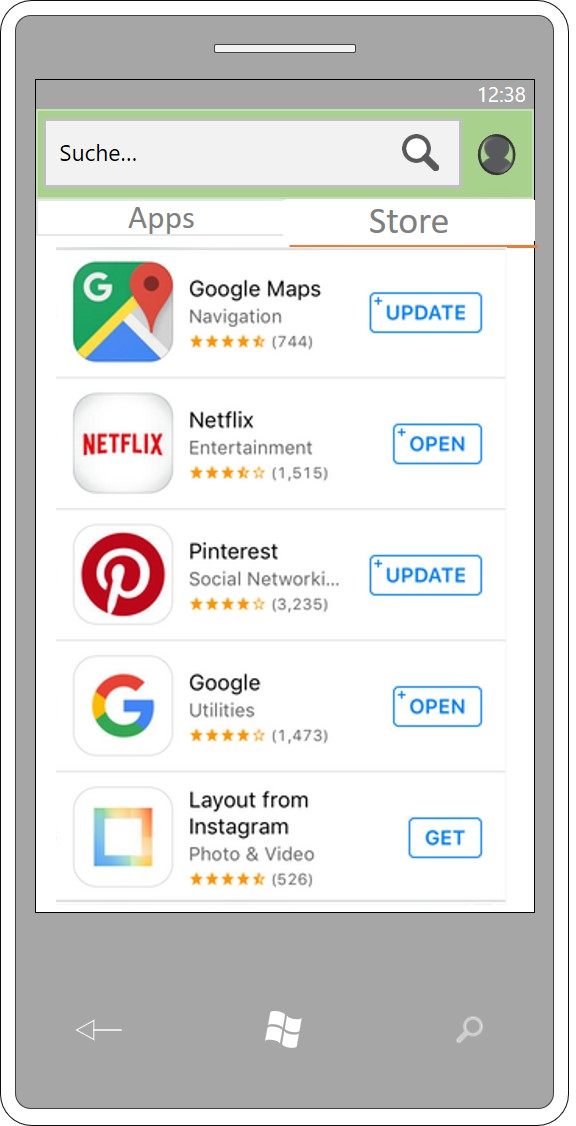
\includegraphics[width=1\linewidth]{Picture/App-Store}
		\caption{Store}
		\label{fig:prototyp1}
	\end{subfigure}%
	\begin{subfigure}{0.32\linewidth}
		\centering
		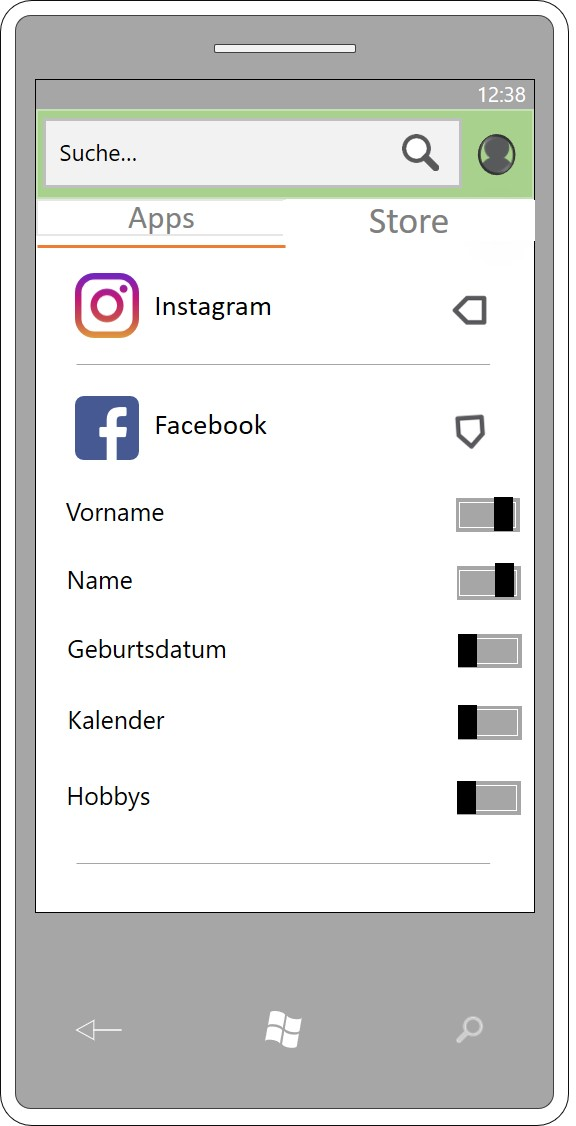
\includegraphics[width=1\linewidth]{Picture/App-Settings}
		\caption{Einstellungen}
		\label{fig:prototyp2}
	\end{subfigure}
	\begin{subfigure}{0.32\linewidth}
		\centering
		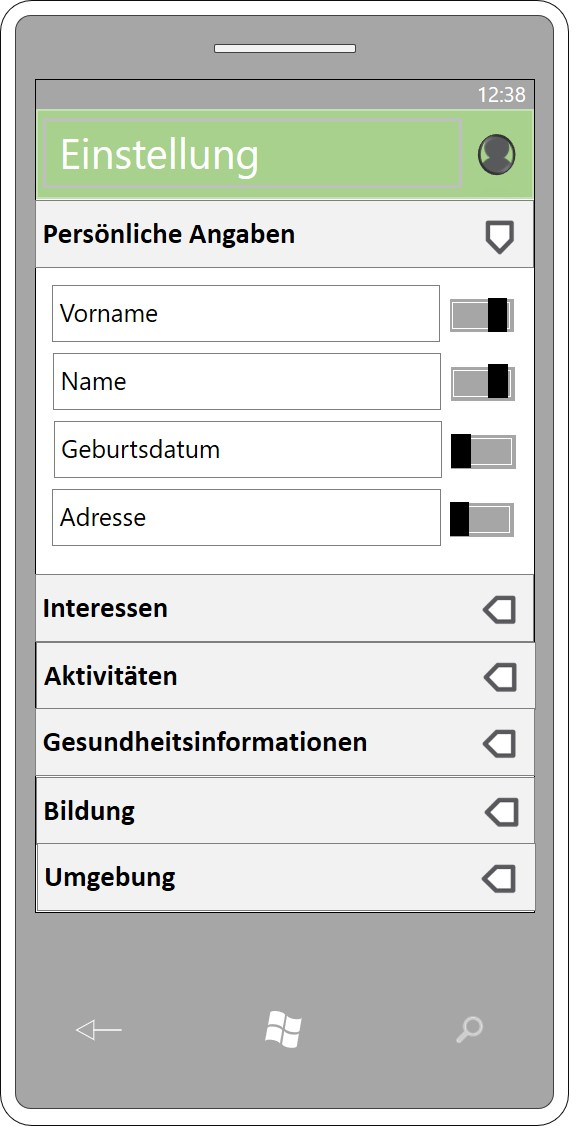
\includegraphics[width=1\linewidth]{Picture/App-Kontext}
		\caption{Nutzer Kontext}
		\label{fig:prototyp3}
	\end{subfigure}%
	\caption{Prototyp der App}
	\label{fig:prototyp}
\end{figure}











